\chapter{State-of-the-art} \label{chap:State_of_the_art}

In the present chapter, a review of the current technology related to the topic of this work will be reviewed.

\section{Morphing aircraft} \label{sec:Morphing_state}

The interest in morphing of the aerodynamic surfaces has accompany aerospace history since the beginning. Since the first heavier-than-air flight in 1903, when the Wright Brothers designed and build the first controlled, sustained flight of a powered heavier-than-air aircraft. Their concept of aircraft did not provide importance to built-in stability but absolute control of the aircraft by the pilot. For this reason, they deliberatively designed their first aircraft with anhedral wing that make it be dynamically unstable to perturbations in sideslip but more maneuverable in the lateral direction. In order to achieve roll control, they decided to incorporate a mechanism that would allow the wings to twist by pulling from cables, as it can be seen in Figure \ref{fig:Wright}. This was the first ever use of morphing of an aerodynamic surface for...

\begin{figure}[!htpb]
  \centering
  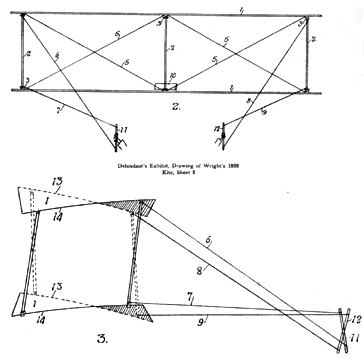
\includegraphics[width=0.8 \textwidth]{WrightBrothers1899Kite}
  \caption[Schematic view of the beam closed section]{Wright 1899 kite: front and side views, with control sticks. Wing-warping is shown in lower view. \cite{Wright}}\label{fig:Wright}
\end{figure}

%NASA morphing proyect  